\chapter{Estudio del Problema Singular}


En esté capítulo se va encuentra el resultado original de esta tesis. Aquí se van aplicar las herramientas desarrolladas en el capitulo anterior al estudio del espectro de un operador singular en un intervalo compacto, encontrando una contradicción al teorema (\ref{eq.heat.expansion}), a su vez se va a generar un scipt de Mathematica que permite graficar distintas aproximaciones a la parte finita de la energía de vacío.

\section{El Operador Singular}


En está sección se estudiará el operador diferencial \ref{operador} obteniendo su espectro y autofunciones
\begin{equation}
\begin{aligned}
    A \phi (x) &= - \partial ^2 _x  \phi(x) + \frac{\alpha}{x} \phi(x) \\[5pt]
    \phi(0) &= \phi(L) = 0 \, .
\end{aligned}
\label{operador}
\end{equation}

Para calcular la {\it función-$\zeta$} solo se van a tener en cuenta los estados ligados, cuyos autovalores están dados por 

\begin{equation}
\begin{aligned}
    A  \phi (x)  &=   \lambda ^2 \phi (x) \\[5pt]
    \lambda \ &\in \ \mathfrak{R} _+ 
    \, ,
\end{aligned}
\label{eq.aut.sin}
\end{equation}
las soluciones LI $ y_1 $ e $ y_2 $ de (\ref{eq.aut.sin}) están dadas por
\begin{equation}
\begin{aligned}
    \phi (x) =
    C[1]
    \underbrace{
     \ e ^{-i \lambda x} \ x \ F _{1} ^{1} (1+\frac{ \alpha}{2 \lambda i },2,2 i \lambda x) } _ {y_1} + 
      C[2] \underbrace{ \ e^{-i \lambda x } \ x \ U (1+\frac{ \alpha}{2 \lambda i },2,2 i \lambda x) } _{y_2} 
    \, ,
\end{aligned}
\label{eq.phi}
\end{equation}
donde $F _1 ^1(a,b,z)$ y $ U(a,b,z)$ son las soluciones LI de la ecuación hypergeométrica
\begin{equation}
    z \ \partial ^2 _z \ \psi (a,b,z) + (b-z) \
    \partial _z \psi (a,b,z)
    -a \ \psi (a,b,z) = 0 \,
\end{equation}
las cuales poseen las expresiones analíticas 
\begin{equation}
\begin{aligned}
	U(a,b,z) &= \frac{1}{\Gamma (a)} 
	\int _0 ^{\infty} e ^{-zt}
	t ^{a-1}
	(1+t) ^{b-a-1}
	dt \\[5pt]
	F _1 ^1 (a,b,z) &= \sum _ {k=0} ^{\infty} 
	\frac{(a) _k}{(b) _k} 
	\frac{z ^k}{k!} 
	\, ,
\end{aligned}
\end{equation}

donde $( \   ) _n$ es el símbolo de Pochhammer. \\



\textbf{Espectro del operador:} \\

Desarrollando $\phi (x)$ alrededor de $x \rightarrow 0$ se obtiene
\begin{align}
\phi (x \rightarrow 0) &=
C[1] ( x + O(x ^2)) + 
C[2] \ x 
\left( 
\frac{1}{  \alpha x  \Gamma ( \frac{ \alpha}{2 i \lambda}  )   }  +
\frac{\log (x) }{\Gamma ( \frac{ \alpha}{2 i \lambda} ) } + Cte + O(x)
\right)
	\nonumber
\\[10pt]
Cte &= 
\frac{
-1 + 2 \gamma + \log ( 2  i \lambda ) + \psi (1 + \frac{ \alpha}{2 i \lambda})
}
{\Gamma (\frac{i \alpha}{2 \lambda})}
\, ,
\label{eq.scat}
\end{align}
de este desarrollo se ve que $y _1 (x \rightarrow 0 ) \rightarrow 0$ e $y _2 (x \rightarrow 0)  \rightarrow
\frac{1}{  \alpha   \Gamma ( \frac{i \alpha}{2 \lambda}  )   } $ , entonces la condición de contorno en $x=0$ fija $C[2] =0$.
Utilizando la condición de contorno en $x=L$ los autovalores están dados por
\begin{equation}
F _1 ^1 (1+\frac{ \alpha}{2 i \lambda},2,2 i \lambda L)  = 0
	\, .
\label{eq.1}
\end{equation}
En la figura (\ref{fig:funcion}) está graficada la función  
\mbox{$ | F _1 ^1 (1+\frac{ \alpha}{2 i \lambda},2,2 i \lambda L) | ^2 $} para   $\alpha=1, \ L=1$. \\

\begin{figure}[h!]
\centering
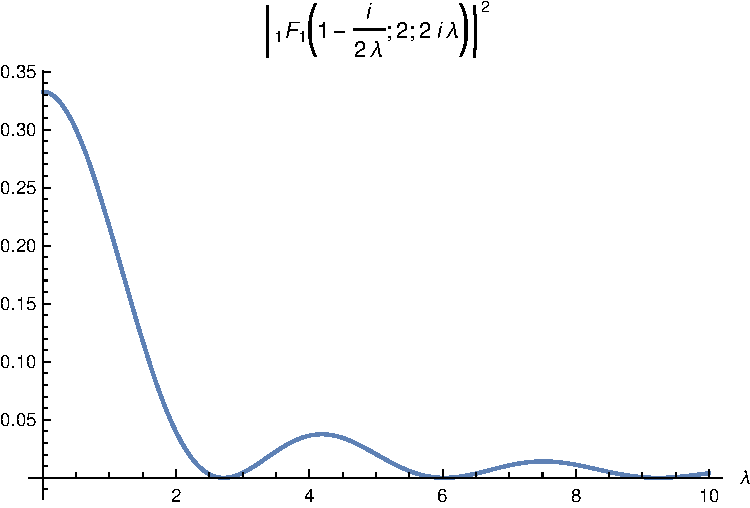
\includegraphics[scale=0.7]{Funcion.pdf}
\caption{En esta imagen se puede ven ver los primeros ceros de la función $| F _1 ^1 (1+\frac{ \alpha}{2 i \lambda},2,2 i \lambda L) | ^2$, para $\alpha=1$ y $L=1$, los cuales representan a los primeros autovalores de $A$.}
\label{fig:funcion}
\end{figure}

\textbf{Desarrollo en serie:} \\

Para determinar los ceros de $F _1 ^1 (1+\frac{ \alpha}{2 i \lambda},2,2 i \lambda L) $ se va a utilizar el desarrollo asintótico $F _1 ^1 (a,b,z)$ a $z \rightarrow \infty$ dado en \cite{Abramowitz:hyper}.
\begin{equation}
\begin{aligned}
    F _1 ^1 (a,b,z) &= \Gamma (b) 
    \left(
    \frac{e^z z ^{a-b} }{\Gamma(a)} * S_1 + \frac{(-z) ^{ -a}}{ \Gamma(b-a)} 
    * S_2
    \right) \\[5pt]
    S _1 &= \sum _{n=0} ^{\infty} \frac{(b-a) _n (1-a) _n}{n!} z ^{-n} \\[5pt]
    S _2 &= \sum _{n=0} ^{\infty} \frac{(a) _n (1+a-b) _n}{n!} (-z) ^{-n}     
		\, .
\end{aligned}
\label{eq.aprox}
\end{equation}
$S_1$ y $S _2$ son las correcciones al orden dominante. Para calcular el polo de la {\it función-$\zeta$} en $s=-1/2$ basta tomar $S _1 = S _2 = 1$ que es lo que se hará a continuación, para conocer los polos mas hallá de $s=-1/2$ o para estudiar la parte finita de $\zeta (-1/2)$ se deben tomar mas términos en $S_1$ y $S _2$, lo cual se hará al final de este capítulo en las secciones \ref{sec.sig.polos} y (REF).

Utilizando (\ref{eq.aprox}) el orden dominante de $F _1 ^1 (1+  \frac{  \alpha}{2 i \lambda} ,2 ,2 i \lambda L  )$ está dado por
\begin{equation}
    i  \frac{e ^{ \frac{\pi}{4} \frac{\alpha}{\lambda} } }{2 \lambda L}
    \left( -
    \frac{e ^{- i \frac{\alpha}{2 \lambda}  \log (2 \lambda L) } e ^{2 i \lambda L} }{\Gamma(1+\frac{ \alpha}{2 i \lambda})} +
    \frac{e ^{  i \frac{\alpha}{2 \lambda}  \log (2 \lambda L) }}               {\Gamma(1-\frac{ \alpha}{2 i \lambda})}
    \right) \\[5pt]  
    =  i  \frac{e ^{ \frac{\pi}{4} \frac{\alpha}{\lambda} } }{2 \lambda L}     M (\lambda) 
    \, ,
\label{eq.completa}
\end{equation}
para obtener la {\it función-$\zeta $} se puede utilizar $M( \lambda)$ así  como cualquier otra función que contenga los mismos ceros que $F _1 ^1 (1+  \frac{  \alpha}{2 i \lambda} ,2 ,2 i \lambda L  )$.

\section{Calculo Asintótico de los autovalores}\label{seq.2.asin}


En está sección se va a utilizar el mismo procedimiento que en en \ref{seq.asin} para calcular la {\it función-$\zeta$}, se va a utilizar un desarrollo de los autovalores para luego usarlos en la definición \ref{def.adim} y así obtener los polos en $s=1/2$ y  $s=-1/2$.

Se van a definir las variables adimensionales: $\mu = \lambda L $ y $\beta = \alpha L$, luego se trabajará con una  $M (\mu)$ de la forma

\begin{equation}
M (\mu) = e ^{\frac{i \beta }{\mu} \log(2 \mu) }
\frac{\Gamma (1 + \frac{ \beta}{2 i \mu})}{\Gamma (1 - \frac{ \beta}{2 i \mu})}
- e ^{2 i \mu}
\, ,
\label{eq.otro.mu}
\end{equation}
en el limite de $\mu  \rightarrow \infty$ se obtiene
\begin{equation}
    M(\mu  \rightarrow \infty) = 
	1 - e ^{2 i \mu}
		\, ,
\end{equation}
de aquí se puede ver que tal como sucedía en \ref{eq.mu} $\mu _n$ queda determinada por un orden dominante y correcciones asintóticas
\begin{equation}
\begin{aligned}
    &\mu _n = n \pi + \epsilon _n \\[5pt]
	&\lim \limits _{n \rightarrow{0}} \epsilon _n  = 0
		\, ,
\end{aligned}
\label{eq.mu2}
\end{equation}
para calcular $\epsilon _n$ se utiliza (\ref{eq.mu2}) en (\ref{eq.otro.mu}), lo cual conduce a
\begin{equation}
	e ^{ i \frac{\beta}{ \mu _n} \log (2 \mu _n)}     
    \frac{\Gamma(1 + \frac{ \beta}{2  i \mu _n} ) }
    {\Gamma(1 -  \frac{ \beta}{2  i \mu _n} )} =    
    e ^{2 i \epsilon _n }
    	\, ,
\label{eq.a.desarrollar}
\end{equation}
sabiendo que $\frac{\log (2 \mu _n)}{2 \mu _n } \rightarrow 0$ en el límite $\mu _n \rightarrow 0$, se va a desarrollar \ref{eq.a.desarrollar} en los límites $ \mu _n \rightarrow \infty $ y $\epsilon _n \rightarrow 0$ obteniendo
\begin{equation}
    \left(
    \sum _{p = 0} ^{\infty} \frac{ \left( i \frac{\beta}{ \mu _n } \log(2 \mu _n ) \right) ^p }{p!}
    \right)
    \left(
	\sum _{q = 0} ^{\infty} \frac{a _q}{\mu _n ^q}
	\right)
    =
    \left(
    \sum _{l = 0} ^{\infty} \frac{( 2 i \epsilon _n)^l}{l !}
    \right)
    	\, ,
\end{equation}
las primeras correcciones a $\epsilon$ se obtienen de
\begin{equation}
\left( 1 + \frac{i \beta}{ \mu _n} \log ( 2 \mu _n) \right) 
\left(1 + \frac{i  \gamma \beta}{ \mu _n} \right)  =
(1 + 2 i \epsilon _n) \, ,
\end{equation}
siendo el termino subdominante $\epsilon _n =  \frac{\beta }{2 n \pi}  \log (2 n \pi)$, lo cual no es suficiente para hallar el polo en $s=-1/2$ ya que existe otro termino que decae como $1/n$, reemplazando $\epsilon _n =  \frac{\beta }{2 n \pi} \log (2 n \pi) + \epsilon '$ en la ecuación anterior, se obtiene:
\begin{equation}
    \epsilon _n =  \frac{\beta }{2 n \pi} \log (2 n \pi) +
                \frac{\gamma \beta}{2 n \pi} +
                O\left(  \frac{1}{n^2} \right)
                	\, .
\end{equation}
Para calcular la {\it función-$\zeta $} se utiliza su definición
\begin{equation}
\begin{aligned}
    \zeta (s) &= \sum _{n=1} ^{\infty} \left( \frac{\lambda _n}{\mu} \right) ^{-2 s}  \\
    & =    ( L \mu ) ^{2 s} \sum _{n=1} ^{\infty} 
    \left( 
    n \pi + \frac{\alpha L }{2 n \pi} \log (2 n \pi) + \frac{\gamma \alpha L}{2 n \pi} +
    O \left( \frac{1}{n^2} \right)
    \right) ^{-2s}
    	\, ,
\end{aligned}
\end{equation}
la cual se puede reescribir como
\begin{equation}
\begin{aligned}
    \zeta _A (s) &= \left( \frac{L \mu }{\pi} \right)  ^{2 s} 
    \sum _{n=1} ^{\infty} n ^{- 2  s} 
    \left(
    	1 + \chi _n 
    	\right) ^{-2 s} \\[5pt]
		 \chi _n &= 
    	\frac{\alpha L  }{2 n^2 \pi ^2} \log (2 n \pi) + 
    	\frac{\gamma \alpha L}{2 n^2 \pi ^2 } +
    	O \left(
    		\frac{1}{n^3} \right) 
    			\, .
\end{aligned}
\end{equation}
Se va a desarrollar el binomio alrededor de  $\chi _n \rightarrow 0$ hasta el termino lineal ya que el termino $\chi _n ^2 $ contribuye a la potencia mas baja en $n ^{-4} $. 
\begin{align}\label{eq.zeta.c}
    \zeta  (s) &= \left( \frac{L \mu}{\pi} \right) ^{2 s}
    \sum _{n=1} ^{\infty} 
    n ^{-2s}
    \left(
    1 - 2 s \chi _n + O \left( \frac{1}{n ^4} \right) \
    \right)   \nonumber \\[5pt]
     &= \left( \frac{L \mu }{\pi} \right) ^{2 s}
    \sum _{n=1} ^{\infty} n ^{-2 s} 
    \left(
    1 - 2s \left(
    \frac{\alpha L }{2 n ^2 \pi ^2} \log ( 2  n \pi) + 
    \frac{\gamma \alpha L }{2 n ^2 \pi ^2} 
	\right) +
    O \left( \frac{1}{n ^{3} }  \right)
    \right) \nonumber \\[5pt]
    &=   \left( \frac{L \mu }{ \pi } \right) ^{2 s}  
    \left( \zeta (2 s) -
	\frac{ s \alpha L}{ \pi ^2} \zeta (2s+2)
	\left(
	    \log (2  \pi ) + \gamma
	\right) + 
    \frac{s \alpha L}{\pi ^2}
	\zeta '(2s+2) \right) \nonumber \\[5pt]
	&\ \ \ \  + \sum _{n=1} ^{\infty} O \left( \frac{1}{n ^{2s+3}} \right) \, .
\end{align}    
Donde sabiendo que $\zeta _R (s) = \frac{1}{s-1} + {\rm Regular} $, el polo en $s=1/2$ queda determinado por

\begin{equation}\label{eq.res.2}
    \zeta  (s \rightarrow 1/2) = \frac{L \mu }{2 \pi} \frac{1}{s-1/2}    
    	\, ,
\end{equation}
lo cual coincide con el resultado general \ref{eq.vol} luego desarrollando \ref{eq.zeta.c} alrededor de $s=-1/2$ se obtiene
\begin{equation}\label{eq.res.1}
    \zeta  (s \rightarrow -1/2 ) =  \frac{\alpha}{8  \pi \mu (s+1/2)^2} +
    \frac{ \alpha ( \gamma  +  \log (2L \mu ) -1 ) }{4  \pi \mu (s+1/2) }  + 
    {\rm Regular}
    	\, ,
\end{equation}
lo cual muestra el primer resultado de esta tesis, la existencia de un polo doble en $\zeta(-1/2)$ lo que está en contradicción con (\ref{eq.heat.expansion}).

\section{Cálculo Utilizando Variable Compleja}\label{seq.2.com}


En la sección anterior se estudio los polos de la {\it función-$\zeta$} en $s=1/2$ y $s=-1/2$ teniendo en cuenta el orden dominante en \ref{eq.aprox}.
En esta sección al igual que en \ref{sec.complejo} se va a expresar la {\it función-$\zeta $} como una integral en el plano complejo, obteniendo coincidencia con (\ref{eq.res.1}) y (\ref{eq.res.2}).

La {\it función-$ \zeta$} queda determinada por
\begin{equation}
\zeta (s) = 
\frac{1}{2 \pi i} 
\int _{\mathcal{C}}
\frac{M ' ( z ) }{ M ( z ) } z ^{-2s} d z = 
\frac{1}{2 \pi i} 
\int _{\mathcal{C}}
\partial _z \ \log 	M(z)  z ^{-2s} \ dz
	\, ,
	\tag{\ref{asd}}
\end{equation}
donde $M (z)$ está definida en (\ref{eq.completa}).

Se va a utilizar el contorno dado por \ref{fig.derecha}. 
Utilizando la parametrización $ z (t) = \pm i t$ sobre los ejes verticales el termino $e ^{2 i \lambda L}$ va a generar un termino exponencialmente creciente/decreciente dependiendo la rama, tirando la parte exponencialmente decreciente y la integral angular se obtiene que la contribución a los polos está dada por 
\begin{comment}
\begin{equation}
\begin{array}{c}
    \zeta  (s) = \\
     \frac{1}{2 \pi i} \int _{\infty} ^{1}
     \frac{ i \alpha }{2 t^2} 
     \left(
      1 + \frac{i \pi}{2} + Ln[2 t] + \psi (1 + \frac{\beta}{2 t})
     \right)
     t ^{-2s}
     e ^{- i \pi s} (i dt) + \\
     \frac{1}{2 \pi i} \int _{\infty} ^{1} 
     \left(
     2 + \frac{\beta}{2 t^2}
     \left(
     1 + \frac{i \pi}{2} - Ln[2 t] - \psi (1+ \frac{\beta}{2 t})
     \right)
     t ^{-2s}
     e ^{ i \pi s} (-i dt)
     \right)     
\end{array}
\end{equation}
\end{comment}

\begin{align}\label{eq.zeta.logs}
    \zeta  (s) =& \\
     & \frac{e^{-i \pi s} \mu ^{2s}}{2 \pi i} \int _{\infty} ^{1}
     \frac{ i \alpha}{2 t^2}
     \left(
     - 1 +  \log (2 L t) + \frac{i \pi}{2}  - \psi \left( 1+\frac{\alpha}{2 t} \right)
     \right)
     t^{-2 s}
      \nonumber
     (i dt) + \\
     & \frac{e^{i \pi s} \mu ^{2s}}{2 \pi i} \int _1 ^{\infty}
	\left(      
     \frac{ i \alpha}{2  t^2}
     \left(
     1 -  \log (2 L t) + \frac{i \pi}{2} + \psi \left( 1 + \frac{\alpha}{2 t} \right)       
     \right)
     + 2 i L
     \right)
     t^{-2 s}
     (-i dt) \nonumber
     	\, .
\end{align}
El término que tiene la potencia mas alta de $t$ va a dar el polo en $s=1/2$ el cual está dado por
\begin{equation}
    \frac{e^{i \pi s} \mu ^{2s} }{2 \pi i }
    \int _1 ^{\infty}
    2 i L    
    t ^{-2 s}
    (-i dt) =  
    \frac{L e^{i \pi s} \mu ^{2s}}{2 \pi i} \frac{1}{s-1/2   }
    	\, ,
\end{equation}
ningún otro termino aportará a este polo, entonces coincidiendo con \ref{eq.res.2} se obtiene
\begin{equation}
    \zeta (s \rightarrow 1/2) = \frac{L \mu }{2 \pi} \frac{1}{s- 1/2 } + Regular
    	\, .
\end{equation}
Una vez calculado este termino, el resto de la integral se puede reescribir como
\begin{align}
	\zeta (s) =&  
		\nonumber \\[5pt]
    & \frac{\alpha \mu ^{2s} }{2 \pi} \ sin(\pi s)
    \int _1 ^{\infty}
    t ^{-2 s-2} 
    \left(
    1 -  \log (2Lt) + \psi \left( 1 + \frac{\alpha}{2t} \right)
    \right) dt \ + 
    	\nonumber \\[5pt]
    &
    \frac{\alpha \mu ^{2s} }{4} 
    Cos(\pi s)
    \int _1 ^{\infty} t^{-2s-2} dt
    	\, ,
\end{align}
donde todos los términos son calculables analíticamente, excepto el que contiene $\psi \left( 1 + \frac{\alpha}{2t} \right)$, para lo cual se desarrolla $\psi \left( 1 + \frac{\alpha}{2t} \right) $ alrededor de $t \rightarrow \infty$ a orden cero, dado que el siguiente orden contribuye al polo en $s = -3/2$

\begin{equation}
    \psi(1 + \frac{\alpha}{2 t}) =
    - \gamma + O \left( \frac{1}{t} \right)
    \, ,
\end{equation}
realizando todas las integrales, la {\it función-$\zeta (s)$} queda determinada por:  
\begin{equation}
\begin{aligned}
    \zeta  (s)  = 
    & \frac{L \mu ^{2 s} e ^{i \pi s}}{2 \pi i} \frac{1}{s-1/2} 
    -\frac{\alpha \mu ^{2s} \sin(\pi s)}{8 \pi} \frac{1}{(s+1/2) ^2} + \\
    & \frac{\alpha \mu ^{2s} sin (\pi s) }{4 \pi } \frac{1 - \gamma -   \log (2 L)}{s+1/2}
    + \frac{\alpha \mu ^{2s} Cos(\pi s)}{8} \frac{1}{s+1/2}
    	\, .
\end{aligned}
\end{equation}
Para calcular el polo en $s=-1/2$ se desarrolla en Serie de Laurent, obteniendo el mismo resultado (\ref{eq.res.1})
\begin{equation}
\begin{aligned}
	\zeta (s \rightarrow -1/2) = 
    &\frac{\alpha}{8 \pi \mu } \frac{1}{(s+1/2)^2} + \\
	&\frac{\alpha ( \gamma  +  \log (2L \mu ) -1 )}{4 \pi \mu } \frac{1}{s+1/2} + \ Regular    
\end{aligned}
\tag{\ref{eq.res.1}}
\end{equation}



\section{Siguientes Polos}\label{sec.sig.polos}


En las secciones \ref{seq.2.com} y \ref{seq.2.asin} se utilizó el termino dominante en el desarrollo de $F _{1} ^{1} (1+\frac{ \alpha}{2 \lambda i },2,2 i \lambda x)$ para obtener los polos en $s=1/2$ y en $s=-1/2$. En esta sección se van a utilizar todos los términos del desarrollo $\ref{eq.aprox}$ para obtener la estructura de polos mas hallá de $s=-1/2$, demostrando que todos son polos simples. 

Se va a calcular la {\it función-$\zeta$} utilizando variable compleja, como en la sección anterior pero con $M ( \lambda )$ dada por


\begin{align}
M( \lambda ) &= 
-
 \frac{e ^{2 i \lambda L } e ^{ - \frac{i \alpha  }{2 \lambda } Ln \left( 2 \lambda L \right) }  }
      { \Gamma \left( 1 + \frac{ \alpha}{2 i \lambda}  \right) } S1 ( \lambda ) +
 \frac{ e ^{   \frac{i \alpha  } {2 \lambda } Ln \left(2 \lambda L \right) } }
      { \Gamma \left( 1 - \frac{ \alpha}{2 i \lambda}  \right)   } S2 ( \lambda )        
      \\[10pt]      
S1 ( \lambda ) &= \sum _{n=0} ^{ \infty }
\frac{\Gamma (1 - \frac{ \alpha}{2 i \lambda} + n )}{\Gamma (1 - \frac{ \alpha}{2 i \lambda})} 
\frac{\Gamma (- \frac{ \alpha}{2 i \lambda} + n )}{\Gamma (- \frac{\alpha}{2 i \lambda})} 
\frac{1}{( 2 i \lambda L ) ^n} = 
1 + \sum _{n=1} ^{\infty} \frac{S ^{(1)} _n (\lambda)}{\lambda ^n} 
	\nonumber
	\\[10pt]
S2 (\lambda ) &= \sum _{n=0 } ^{\infty}
\frac{ \Gamma ( 1 + \frac{ \alpha}{2 i \lambda } + n ) }{\Gamma ( 1 + \frac{ \alpha}{2 i \lambda } )}
\frac{\Gamma ( \frac{ \alpha }{2 i \lambda} + n )}{\Gamma ( \frac{ \alpha }{2 i \lambda} )}
\frac{1}{( - 2 i \lambda L ) ^n} = 
1 + \sum _{n=1} ^{\infty} \frac{S ^{(2)} _n (\lambda)}{\lambda ^n}
\nonumber
\label{larga}
\end{align}

Donde $S _n ^{(1,2)}$ son un polinomios de potencias negativas, donde el orden mas bajo es 1 y el mas alto $\lambda ^n$. 


Al igual que en \ref{seq.2.com} al integrar sobre los ejes verticales va a haber una parte exponencialmente creciente o decreciente, tirando los términos exponencialmente decrecientes se obtiene
\begin{align}
\log ( M ( \lambda = i t ) ) &=   \log (S2) + 
\frac{i \alpha }{2 \lambda}  \log (2 \lambda L) - 
 \log \left( \Gamma \left( 1 - \frac{ \alpha}{2 i \lambda} \right) \right) \\ 
\log ( M ( \lambda=-i t ) ) &=  \log (S1) -  
\frac{i \alpha }{2 \lambda}  \log ( 2 \lambda L ) - 
 \log \left( \Gamma \left( 1 + \frac{ \alpha}{2 i \lambda} \right) \right) +
2 i \lambda L  \nonumber
	\,	,
\end{align}
donde la única diferencia con los logaritmos utilizados para llegar a (\ref{eq.zeta.logs}) es la contribución de los términos $\log ( S1 )$ y $ \log ( S2) $.

Teniendo en cuenta solo los términos que contribuyen a los polos en  $s < -1/2$ se obtiene
\begin{equation}
\begin{aligned}
 \zeta  (s) =& \\[10pt]
& \frac{e ^{- i \pi s} \mu ^{2s } }{2 \pi}
\int _{\infty} ^{1} t ^{-2s } 
		\frac{S2' (it)}{S2 (it)}
		d t
	- 
\frac{e ^{i \pi s} \mu ^{2s}}{2 \pi}
\int _{1} ^{\infty} t ^{-2s } 
	\frac{S1' (-it)}{S1(-it)}
	d t +
	 \\[10pt]
	&  \frac{\alpha \mu ^{2s} }{2 \pi }	\sin ( \pi s)  \int _1 ^{\infty}
	t ^{-2s-2} \left( \psi \left( 1 + \frac{\alpha}{2 t}\right) + \gamma \right) dt 
		\, .
\end{aligned}
\end{equation}
Utilizando que  $\frac{S1' (-it)}{S1 (-i t)} = - \frac{S2 ' (i t)}{S2(it)} = \frac{S'(t)}{S(t)}  $ se puede reescribir lo anterior como
\begin{equation}
\begin{aligned}
\zeta  (s) =&  \\[5pt]
&
\frac{\alpha \mu ^{2s} sin( \pi s )}{2 \pi } \int _{1} ^{\infty} 
t ^{-2s-2} \left( \psi (1 + \frac{\alpha}{2 t}) + \gamma \right) dt -\\[5pt]
&   \frac{i \mu ^{2s}  sin (\pi s)}{\pi} \int _1 ^{\infty} t ^{-2s} \frac{S'(t)}{S(t)} dt 
	\, ,
\end{aligned}
\end{equation}
de aquí se puede que solo van a existir polos simples en los semienteros negativos dado que $\sin (\pi s)$ posee ceros simples en los enteros negativos, lo cual coincide con el caso regular.

En vez de desarrollar en serie $S'(t) / S (t)$ se desarrolla el Logaritmo y se le toma la derivada para luego evaluar en $\lambda \rightarrow -i t$, lo cual nos permite controlar el orden del desarrollo.

\begin{equation}
\begin{aligned}
\frac{S'( \lambda)}{S( \lambda )} &\approx 
\partial _{\lambda} Log \left(
								1 + \sum _{n=1} ^{N-1}  \frac{S _n}{\lambda ^n}
								\right) =
\partial _{\lambda} 
\sum _{m = 1} ^{N/2} 
	\left(
	\frac{(-1) ^{m+1} }{m}
	\left(
		\sum _{n=1} ^{N-1} \frac{S _n}{\lambda ^n}
		\right) ^m 
	\right)  \\[10pt]
	&=
\left(								
	\sum _{l = 1} ^{N-1} 
	\frac{S' _l}{\lambda ^l} - l \frac{S _l}{\lambda ^{l+1}}
	\right)							
\left(
	\sum _{m = 1} ^{N/2} (-1) ^{m+1} 
	\left(
			\sum _{n=1} ^{N-1} \frac{S _n}{\lambda ^n}
			\right) ^{m-1}		
	\right)
\end{aligned}	
\end{equation}



Este desarrollo de Taylor es correcto hasta el orden N (en caso de que N sea semientero hay que tomarle la parte entera), tiene la ventaja de poder ser calculado explícitamente, los primeros términos de $\frac{S'(t)}{S(t)}$ son:

\begin{equation}
\frac{S'(t)}{S(t)} = 
\frac{i \alpha}{2 L t^3} -
\frac{3 i (L \alpha ^2 - 2 \alpha)}{8 L^2 t ^4}
\end{equation}




Con este desarrollo puedo encontrar el polo en $s=-3/2$.
\begin{equation}
\zeta _A (s \rightarrow -3/2) = 
\frac{L ^2 \alpha  ^3 \psi ^{(2)} (1) + 12   \alpha  - 6 L \alpha ^2}{32 L^2 \pi \mu ^3}
\frac{1}{s+3/2}
\end{equation}

Para seguir calculando la estructura de polos, basta con seguir desarrollando las funciones $S(t)$ y $\psi (1 + \frac{\alpha}{2 t})$.

%Estos comentarios tienen las contribuciones de la parte finita
\begin{comment}
Las primeras 3 integrales se pueden realizar analíticamente de manera sencilla, dado que son todas series de potencias, la integral angular va a tener que ser evaluada numéricamente dado que es de la forma (parametrizando $\lambda = e ^{i \theta}$ y llamando $M_c$ a todo el termino adentro del Logaritmo) :

\begin{equation}
\begin{array}{c}

\frac{1}{2 \pi i} \int _{\pi /2 } ^{- \pi /2} 
\frac{e ^{-2 s i \theta} d \theta}{M [e ^{i \theta}]} \\

\Bigg[

\frac{
e ^{- \frac{i \alpha (Ln[2 L] + i \theta)}{2 e ^{i \theta} }} e ^{2 i L e ^{i \theta}}
}{\Gamma \left( 1 - \frac{i \alpha}{2 e ^{i \theta}} \right)}
	\left(
		\left(
			2 i L -
			\frac{i \alpha}{2 e ^{2 i \theta} } + 
			\frac{i \alpha( Ln[2 L ] + e ^{i \theta} ) }{2 e^{2 i \theta}}
			- \frac{i \alpha \psi \left( 1 - \frac{i \alpha}{2 e ^{i \theta}}\right)}
				   {2 e ^{2 i \theta}}
			\right) S1 [e ^{i \theta}] +
		S1 ' [e ^{i \theta }]
		\right)
  \\

- \frac{
e ^{ \frac{i \alpha (Ln[2 L] + i \theta)}{2 e ^{i \theta} }}
}{\Gamma \left( 1 + \frac{i \alpha}{2 e ^{i \theta}} \right)}
	\left(
		\left(
			\frac{i \alpha}{2 e ^{2 i \theta} } - 
			\frac{i \alpha( Ln[2 L ] + e ^{i \theta} ) }{2 e^{2 i \theta}}
			+ \frac{i \alpha \psi \left( 1 + \frac{i \alpha}{2 e ^{i \theta}}\right)}
				   {2 e ^{2 i \theta}}
			\right) S2 [e ^{i \theta}] +
		S'2 [e ^{i \theta }]
		\right)


\Bigg]

\end{array}
\end{equation}

La cual va a dar una constante independiente de $\lambda$ y se puede calcular numéricamente.


A la hora de calcular los términos de la forma $S'/S$ hay que tener en cuenta hasta que orden hay que llevar el numerado y el denominador para poder ser consistente con la expansión en serie.

\begin{equation}
\begin{array}{c}
\frac{S'(x)}{S(x)} =
\frac{
		- \sum _{n=1} ^{\infty} \frac{n a_n}{x ^{n+1}}
      }
      {
		1 + \sum _{m=1} ^{\infty} \frac{a _n}{x ^{n}}
            } =
            

\left(
	    - \sum _{n=1} ^{\infty} \frac{n a_n}{x ^{n+1}}
		\right)
\sum _{p =0} ^{\infty}
		\left(
			    \sum _{m=1} ^{\infty} \frac{a _n}{x ^{n}}
	    		\right) ^{p}
\end{array}
\end{equation}

Donde se puede hacer el producto de Cauchy para tener la solución exacta de hasta que términos hay que desarrollar $S,S'$ y la Serie Geométrica.
\end{comment}
\begin{comment}
\begin{equation}
\frac{1 }{2 \pi i}
\int _{circulo} \lambda ^{-2s } \partial \lambda \ Ln \left[
					\frac{e ^{\frac{i \alpha  \log ( 2 \lambda L )}{2 \lambda}} e ^{2 i \lambda L} S1}
					{\Gamma \left( 1 - \frac{i \alpha}{2 \lambda} \right)} - 
					\frac{e ^{\frac{-i \alpha  \log (2 \lambda L )}{2 \lambda}} S2}
					{\Gamma \left( 1 + \frac{i \alpha}{2 \lambda} \right)}					
					\right] d \lambda
\end{equation}
\end{comment}


\section{Cálculo de la energía de vacío}

La energía de vacío queda definida por la ecuación: 

\begin{equation}
    E _0 = \frac{\mu }{2}  
    \zeta _A \left( - 1/2 \right) 
\end{equation}

Utilizando el desarrollo de $\zeta _A (s \rightarrow -1/2)$ en (\ref{eq.desarrollo}), se obtiene para la energía de vacío:

\begin{equation}
E _0 = \frac{1}{2} \left(
				\frac{\alpha}{8 \pi  } \frac{1}{(s+1/2)^2} + 
				\frac{\alpha ( \gamma  +  \log (2L \mu ) -1 )}{4 \pi  } \frac{1}{s+1/2} +
				\ Regular
				\right)
\end{equation}

 
